\documentclass[12pt]{beamer}
\usepackage{../Estilos/BeamerFC}
\usepackage{../Estilos/ColoresLatex}
\usepackage{courier}
\usepackage{listingsutf8}
\usepackage{listings}
\usepackage{xcolor}
\usepackage{textcomp}
\usepackage{color}
\definecolor{deepblue}{rgb}{0,0,0.5}
\definecolor{brown}{rgb}{0.59, 0.29, 0.0}
\definecolor{OliveGreen}{rgb}{0,0.25,0}
% \usepackage{minted}

\DeclareCaptionFont{white}{\color{white}}
\DeclareCaptionFormat{listing}{\colorbox{gray}{\parbox{0.98\textwidth}{#1#2#3}}}
\captionsetup[lstlisting]{format=listing,labelfont=white,textfont=white}
\renewcommand{\lstlistingname}{Código}


\definecolor{Code}{rgb}{0,0,0}
\definecolor{Keywords}{rgb}{255,0,0}
\definecolor{Strings}{rgb}{255,0,255}
\definecolor{Comments}{rgb}{0,0,255}
\definecolor{Numbers}{rgb}{255,128,0}

\makeatletter

\newif\iffirstchar\firstchartrue
\newif\ifstartedbyadigit
\newif\ifprecededbyequalsign

\newcommand\processletter
{%
  \ifnum\lst@mode=\lst@Pmode%
    \iffirstchar%
        \global\startedbyadigitfalse%
      \fi
      \global\firstcharfalse%
    \fi
}

\newcommand\processdigit
{%
  \ifnum\lst@mode=\lst@Pmode%
      \iffirstchar%
        \global\startedbyadigittrue%
      \fi
      \global\firstcharfalse%
  \fi
}

\lst@AddToHook{OutputOther}%
{%
  \lst@IfLastOtherOneOf{=}
    {\global\precededbyequalsigntrue}
    {}%
}

\lst@AddToHook{Output}%
{%
  \ifprecededbyequalsign%
      \ifstartedbyadigit%
        \def\lst@thestyle{\color{orange}}%
      \fi
    \fi
  \global\firstchartrue%
  \global\startedbyadigitfalse%
  \global\precededbyequalsignfalse%
}

\lstset{ 
language=Python,                % choose the language of the code
basicstyle=\footnotesize\ttfamily,       % the size of the fonts that are used for the code
numbers=left,                   % where to put the line-numbers
numberstyle=\scriptsize,      % the size of the fonts that are used for the line-numbers
stepnumber=1,                   % the step between two line-numbers. If it is 1 each line will be numbered
numbersep=5pt,                  % how far the line-numbers are from the code
backgroundcolor=\color{white},  % choose the background color. You must add \usepackage{color}
showspaces=false,               % show spaces adding particular underscores
showstringspaces=false,         % underline spaces within strings
showtabs=false,                 % show tabs within strings adding particular underscores
frame=single,   		% adds a frame around the code
tabsize=2,  		% sets default tabsize to 2 spaces
captionpos=t,   		% sets the caption-position to bottom
breaklines=true,    	% sets automatic line breaking
breakatwhitespace=false,    % sets if automatic breaks should only happen at whitespace
escapeinside={| |},  % if you want to add a comment within your code
stringstyle =\color{OliveGreen},
otherkeywords={as, np.array, np.concatenate, np.linspace, linspace, interpolate.interp1d, kind, plt.plot, .copy, np.arange, np.cos, np.pi, lw, ls, label, splrep, splev, plt.legend, loc, plt.title, plt.ylim, plt.show, sign, math.ceil, math.log, np.sqrt, np.exp, np.zeros, plt.xlabel, plt.ylabel, plt.xlim, np.identity, random, np.dot, np.outer, np.diagonal },             % Add keywords here
keywordstyle = \color{blue},
commentstyle = \color{darkcerulean},
identifierstyle = \color{black},
literate=%
         {á}{{\'a}}1
         {é}{{\'e}}1
         {í}{{\'i}}1
         {ó}{{\'o}}1
         {ú}{{\'u}}1
%
%keywordstyle=\ttb\color{deepblue}
%fancyvrb = true,
}

\lstdefinestyle{FormattedNumber}{%
    literate={0}{{\textcolor{red}{0}}}{1}%
             {1}{{\textcolor{red}{1}}}{1}%
             {2}{{\textcolor{red}{2}}}{1}%
             {3}{{\textcolor{red}{3}}}{1}%
             {4}{{\textcolor{red}{4}}}{1}%
             {5}{{\textcolor{red}{5}}}{1}%
             {6}{{\textcolor{red}{6}}}{1}%
             {7}{{\textcolor{red}{7}}}{1}%
             {8}{{\textcolor{red}{8}}}{1}%
             {9}{{\textcolor{red}{9}}}{1}%
             {.0}{{\textcolor{red}{.0}}}{2}% Following is to ensure that only periods
             {.1}{{\textcolor{red}{.1}}}{2}% followed by a digit are changed.
             {.2}{{\textcolor{red}{.2}}}{2}%
             {.3}{{\textcolor{red}{.3}}}{2}%
             {.4}{{\textcolor{red}{.4}}}{2}%
             {.5}{{\textcolor{red}{.5}}}{2}%
             {.6}{{\textcolor{red}{.6}}}{2}%
             {.7}{{\textcolor{red}{.7}}}{2}%
             {.8}{{\textcolor{red}{.8}}}{2}%
             {.9}{{\textcolor{red}{.9}}}{2}%
             {\ }{{ }}{1}% handle the space
         ,%
          %mathescape=true
          escapeinside={__}
          }



\usetheme{Dresden}
\usecolortheme{seahorse}
%\useoutertheme{default}
\setbeamercovered{invisible}
% or whatever (possibly just delete it)
\setbeamertemplate{section in toc}[sections numbered]
\setbeamertemplate{subsection in toc}[subsections numbered]
\setbeamertemplate{subsection in toc}{\leavevmode\leftskip=3.2em\rlap{\hskip-2em\inserttocsectionnumber.\inserttocsubsectionnumber}\inserttocsubsection\par}
\setbeamercolor{section in toc}{fg=blue}
\setbeamercolor{subsection in toc}{fg=blue}
\setbeamercolor{frametitle}{fg=blue}
\setbeamertemplate{caption}[numbered]

\setbeamertemplate{footline}
\beamertemplatenavigationsymbolsempty
\setbeamertemplate{headline}{}

\makeatletter
\setbeamercolor{section in foot}{bg=gray!30, fg=black!90!orange}
\setbeamercolor{subsection in foot}{bg=blue!30!yellow, fg=red}
\setbeamertemplate{footline}
{
  \leavevmode%
  \hbox{%
  \begin{beamercolorbox}[wd=.333333\paperwidth,ht=2.25ex,dp=1ex,center]{section in foot}%
    \usebeamerfont{section in foot} \insertsection
  \end{beamercolorbox}}%
  \begin{beamercolorbox}[wd=.333333\paperwidth,ht=2.25ex,dp=1ex,center]{subsection in foot}%
    \usebeamerfont{subsection in foot}  \insertsubsection
  \end{beamercolorbox}%
  \begin{beamercolorbox}[wd=.333333\paperwidth,ht=2.25ex,dp=1ex,right]{date in head/foot}%
    \usebeamerfont{date in head/foot} \insertshortdate{} \hspace*{2em}
    \insertframenumber{} / \inserttotalframenumber \hspace*{2ex} 
  \end{beamercolorbox}}%
  \vskip0pt%
\makeatother 

\makeatletter
\patchcmd{\beamer@sectionintoc}{\vskip1.5em}{\vskip0.8em}{}{}
\makeatother

%\usefonttheme{serif}

\title{Técnicas de Interpolación}
\subtitle{Tema 2 - Operaciones matemáticas básicas}
\author{M. en C. Gustavo Contreras Mayén}
\date{}

\begin{document}
\maketitle

\section*{Contenido}
\frame{\tableofcontents[currentsection, hideallsubsections]}

\section{Interp. Lagrange}
\frame{\tableofcontents[currentsection, hideothersubsections]}
\subsection{Resolviendo con python}

\begin{frame}
\frametitle{Ejercicio de interpolación}
A partir de la siguiente tabla de datos:
\pause
\begin{center}
\renewcommand{\arraystretch}{0.9}
\begin{tabular}{c | c | c | c | c}
$x$ & $1$ & $2$ & $3$ & $4$ \\ \hline
$P (x)$ & $0.671$ & $0.620$ & $0.567$ & $0.512$ \\
\end{tabular}
\end{center}
\pause
Usa el algoritmo de interpolación de Lagrange con un polinomio de grado $n = 3$, para estimar el valor de $P (x)$ en los siguientes puntos:
\begin{align*}
x = 1.5, 2.5, 3.5
\end{align*}
\end{frame}
\begin{frame}
\frametitle{Corroborar los resultados obtenidos}
Aunque el enunciado no lo solicite directamente, podemos avanzar en la comprobación de los resultados si:
\setbeamercolor{item projected}{bg=aqua,fg=applegreen}
\setbeamertemplate{enumerate items}{%
\usebeamercolor[bg]{item projected}%
\raisebox{1.5pt}{\colorbox{bg}{\color{fg}\footnotesize\insertenumlabel}}%
}
\begin{enumerate}[<+->]
\item Graficamos el conjunto de datos de la tabla y los valores que nos devuelve la interpolación.
\item Calculamos el polinomio de interpolación y lo incluimos en la gráfica anterior.
\end{enumerate}
\end{frame}
\begin{frame}
\frametitle{Corroborar los resultados obtenidos}
De esta manera veremos la tendencia de los datos de interpolación con los datos de la tabla, si alguno no corresponde, entonces tendremos que revisar nuestro código.
\end{frame}
\begin{frame}[allowframebreaks, fragile]
\frametitle{Solución al problema}
\begin{lstlisting}[caption=Código para la interpolación de Lagrange]
import numpy as np

n = 3

x0 = np.array([1.5, 2.5, 3.5])
x = np.array([1., 2., 3., 4.])
f = np.array([0.671, 0.620, 0.567, 0.512])

for k in x0:
    yres = 0
    for i in range(0, n + 1):
        z = 1.0
        for j in range(0, n + 1):
            if i != j:
                z = z * (k - x[j])/(x[i] - x[j])
        yres = yres + z * f[i] 
    
    print ('El polinomio evaluado en P ({0:}) = {1:}'.format(k,  yres))
\end{lstlisting}
\end{frame}
\begin{frame}[fragile]
\frametitle{Solución (en la terminal y con una gráfica)}
\begin{table}
\centering
\renewcommand{\arraystretch}{0.9}
\begin{tabular}{c | l}
$x$ & $P (x)$ \\
\hline $1$   & $0.671$ \\
\hline $1.5$ & $0.64575$ \\
\hline $2$   & $0.620$ \\
\hline $2.5$ & $0.59375$ \\
\hline $3$   & $0.567$ \\
\hline $3.5$ & $0.53975$ \\
\hline $4$   & $0.512$
\end{tabular}
\end{table}
\end{frame}
\begin{frame}
\frametitle{Solución con una gráfica}
\begin{figure}
	\centering
	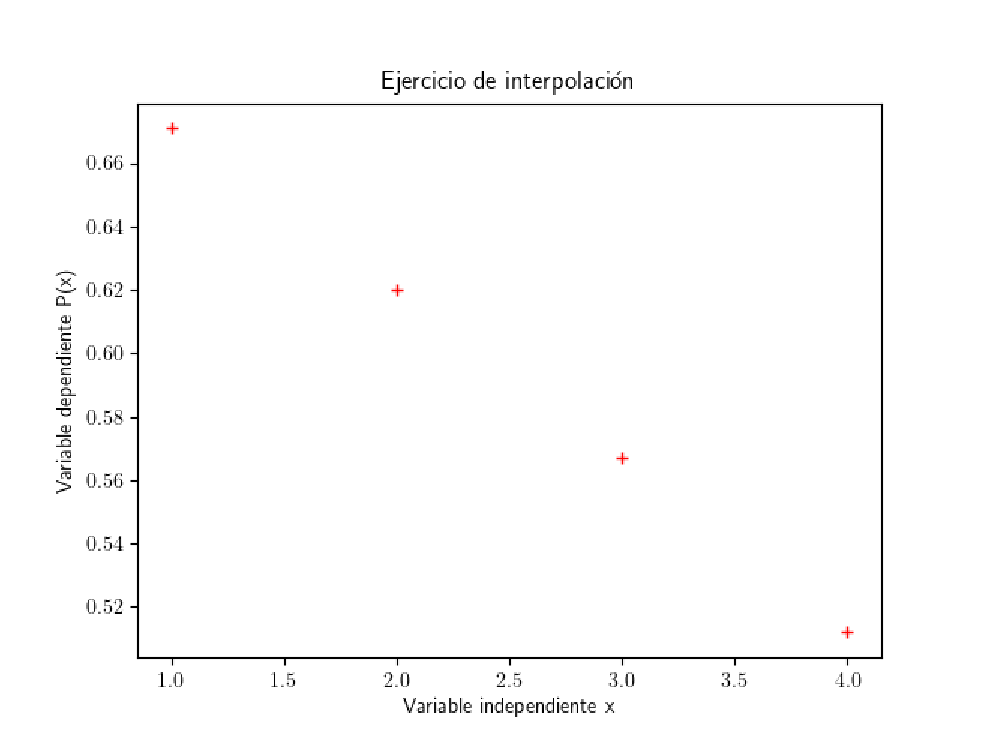
\includegraphics[scale=0.58]{Imagenes/Ejercicio_Interpolacion_01.eps}
	%\caption{Gráfica con los datos experimentales}
\end{figure}
\end{frame}
\begin{frame}
\frametitle{Solución con una gráfica}
\begin{figure}
	\centering
	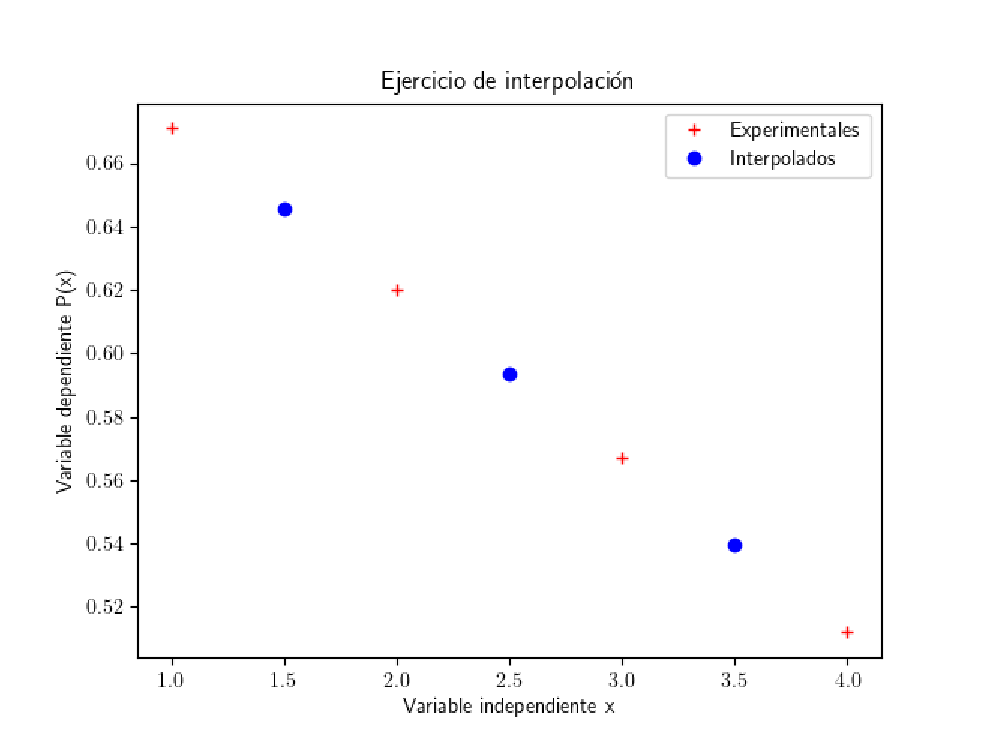
\includegraphics[scale=0.58]{Imagenes/Ejercicio_Interpolacion_02.eps}
	%\caption{Datos experimentales y el valor de interpolación -bola azul-}
\end{figure}
\end{frame}
\begin{frame}
\frametitle{Obteniendo el polinomio de interpolación}
Una vez que hemos obtenidos los valores de interpolación, contamos con más elementos que nos favorecerán para obtener el polinomio de interpolación, ocupando las funciones de \python.
\end{frame}
\begin{frame}
\frametitle{Usando \python{} para interpolar}
En la librería \funcionazul{scipy} (\textit{Scientific python}) cuenta con un módulo para interpolación: \pause \funcionazul{interpolate}, dentro del cual se tiene la función \pause \funcionazul{interp1d}.
\end{frame}
\begin{frame}
\frametitle{La función \texttt{interp1d}}
Se necesitan dos arreglos: $x$ e $y$ con valores que se utilizan para aproximar alguna función $f: \, y = f (x)$.
\\
\bigskip
\pause
Este objeto devuelve una función cuyo método usa la interpolación para calcular el valor de nuevos puntos.
\end{frame}
\begin{frame}
\frametitle{Parámetros necesarios}
Se requieren tres parámetros como mínimo para utilizar esta función:
\pause
\setbeamercolor{item projected}{bg=ao(english),fg=aureolin}
\setbeamertemplate{enumerate items}{%
\usebeamercolor[bg]{item projected}%
\raisebox{1.5pt}{\colorbox{bg}{\color{fg}\footnotesize\insertenumlabel}}%
}
\begin{enumerate}[<+->]
\item Un arreglo unidimensional $x$.
\item Un arreglo $y$,
\item \textit{kind}: Especifica el tipo de interpolación como una cadena: \textit{linear, quadratic, cubic} (entre otros). El valor por defecto es \textit{linear}.
\end{enumerate}
\end{frame}
\begin{frame}
\frametitle{Usando los datos}
Haremos uso de los datos de la tabla y los datos que nos devolvió la interpolación de Lagrange.
\\
\bigskip
\pause
Para ello debemos de concatenar los objetos \textit{narray} de numpy, tanto para el eje $x$ como para el eje $y$.
\end{frame}
\begin{frame}[fragile]
\frametitle{Uniendo los arreglos}
Usaremos la función de numpy: \funcionazul{concatenate}:
\begin{lstlisting}[caption=Uniendo los arreglos]
poli_x = np.concatenate([x, x0])

poli_y = np.concatenate([f, datos])
\end{lstlisting}
\end{frame}
\begin{frame}[fragile]
\frametitle{Definiendo el polinomio de interpolación}
Vamos a ocupar un intervalo de $[1, 4]$ para evaluar el polinomio, que serán los valores en el eje $x$ para la interpolación con la función \funcionazul{interp1d}.
\\
\bigskip
\pause
El ejercicio pide una interpolación con un polinomio de orden $3$, por lo que en el parámetro \funcionazul{kind} se debe de especificar el valor: \textit{cubic}.
\end{frame}
\begin{frame}[fragile]
\frametitle{Definiendo el polinomio de interpolación}
\begin{lstlisting}[caption=Definiendo el polinomio]
from scipy import interpolate

x1 = np.linspace(1, 4)

interp_1 = interpolate.interp1d(poli_x, poli_y, kind='cubic')

y1 = interp_1(x1)
\end{lstlisting}
\end{frame}
\begin{frame}
\frametitle{Ubicando los elementos del código}
Recuerda que hay que colocar las partes del código de manera consistente, es decir:
\setbeamercolor{item projected}{bg=ao,fg=white}
\setbeamertemplate{enumerate items}{%
\usebeamercolor[bg]{item projected}%
\raisebox{1.5pt}{\colorbox{bg}{\color{fg}\footnotesize\insertenumlabel}}%
}
\begin{enumerate}[<+->]
\item La llamada al módulo \funcionazul{interpolate}, debe de quedar al inicio del código.
\item Las variables $x1$, $interp\_1$ y $y1$ deben de quedar antes de la rutina de graficación.
\item La siguiente instrucción para la gráfica queda en el apartado para las otras gráficas.
\end{enumerate}
\end{frame}
\begin{frame}[fragile]
\frametitle{Datos para graficar}
Como ya tenemos un conjunto de datos del mismo tamaño, procedemos a graficar los mismos en una rutina de graficación que ya conocemos:
\pause
\begin{lstlisting}[caption=Graficando los datos de interpolación]
plt.plot(x1, y1, 'm', label='Polinomio interp.')
\end{lstlisting}
\end{frame}
\begin{frame}
\frametitle{Solución con una gráfica}
\begin{figure}
    \centering
    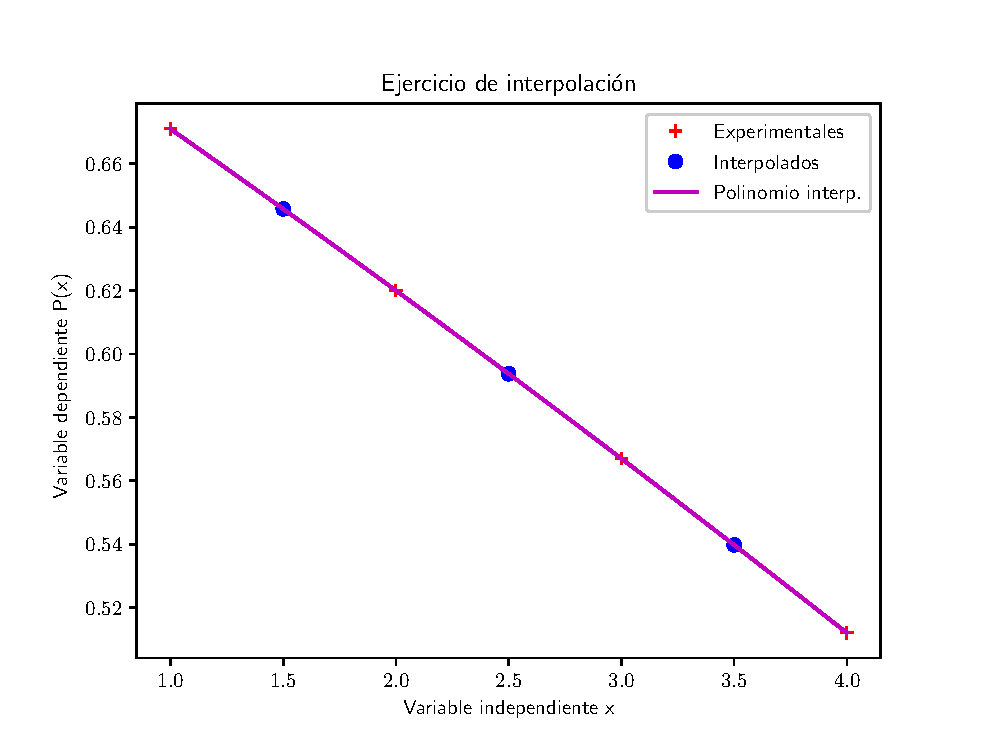
\includegraphics[scale=0.58]{Imagenes/Ejercicio_Interpolacion_03.eps}
\end{figure}
\end{frame}
    

\section{Ejercicios a cuenta}
\frame{\tableofcontents[currentsection, hideothersubsections]}
\subsection{Ejercicio 1}

\begin{frame}
\frametitle{Ejercicio 1}
\setbeamercolor{item projected}{bg=blue,fg=white}
\setbeamertemplate{enumerate items}{%
\usebeamercolor[bg]{item projected}%
\raisebox{1.5pt}{\colorbox{bg}{\color{fg}\footnotesize\insertenumlabel}}%
}
\begin{enumerate}[<+->]
\item Ajusta $x \, \sin(x)$ en el intervalo $[0, \, \pi/2]$ con un polinomio de interpolación de Lagrange de orden $n = 4$, utilizando puntos con igual separación, necesitaremos entonces $n + 1 = 5$ puntos.
\\
\bigskip
Calcula el error de cada interpolación en cada incremento de $\pi/16$, y genera una gráfica.
\seti
\end{enumerate}
\end{frame}
\begin{frame}[fragile]
\frametitle{Hints para resolver los ejercicios}
Tomemos en cuenta lo siguiente:
\setbeamercolor{item projected}{bg=lava,fg=white}
\setbeamertemplate{enumerate items}{%
\usebeamercolor[bg]{item projected}%
\raisebox{1.5pt}{\colorbox{bg}{\color{fg}\footnotesize\insertenumlabel}}%
}
\begin{enumerate}[<+->]
\item Hay que dividir el intervalo $[0, \pi/2]$ en cinco espacios.
\item Se evalúa la función $x \: sin (x)$ en el conjunto de puntos que obtuvimos.
\item Creamos un conjunto de puntos para ajustar con el método de Lagrange.
\item La manera más fácil es con un \texttt{numpy.linspace}.
\end{enumerate}
\end{frame}    
\begin{frame}
\frametitle{Solución Ejercicio 1}
\begin{figure}
	\centering
	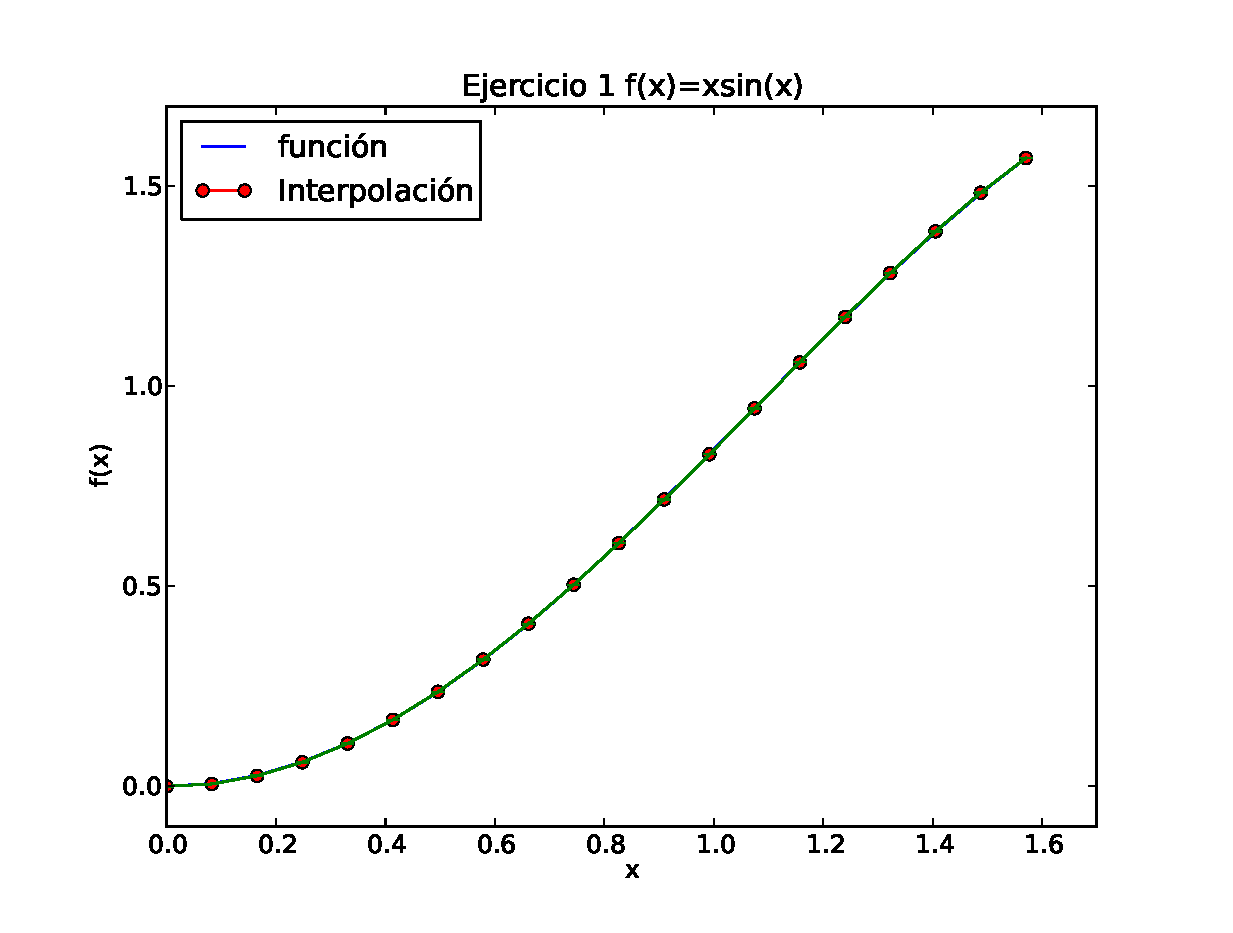
\includegraphics[scale=0.45]{Imagenes/ejercicioTema21_1.eps} 
\end{figure}
\end{frame}


\subsection{Ejercicio 2}

\begin{frame}
\frametitle{Ejercicio 2}
\setbeamercolor{item projected}{bg=blue,fg=white}
\setbeamertemplate{enumerate items}{%
\usebeamercolor[bg]{item projected}%
\raisebox{1.5pt}{\colorbox{bg}{\color{fg}\footnotesize\insertenumlabel}}%
}
\begin{enumerate}
\conti
\item Ajusta $\sin(x)$ en $[0, \, 2\pi]$ con el polinomio de interpolación de Lagrange de orden $n = 4$ y $n = 8$, utilizando puntos con igual separación ($5$ y $9$ puntos respectivamente). 
\\
\bigskip
Grafica los polinomios de interpolación junto con $\sin(x)$ y las distribuciones de sus errores.
\end{enumerate}
\end{frame}
\begin{frame}
\frametitle{Solución Ejercicio 2}
\begin{figure}
	\centering
	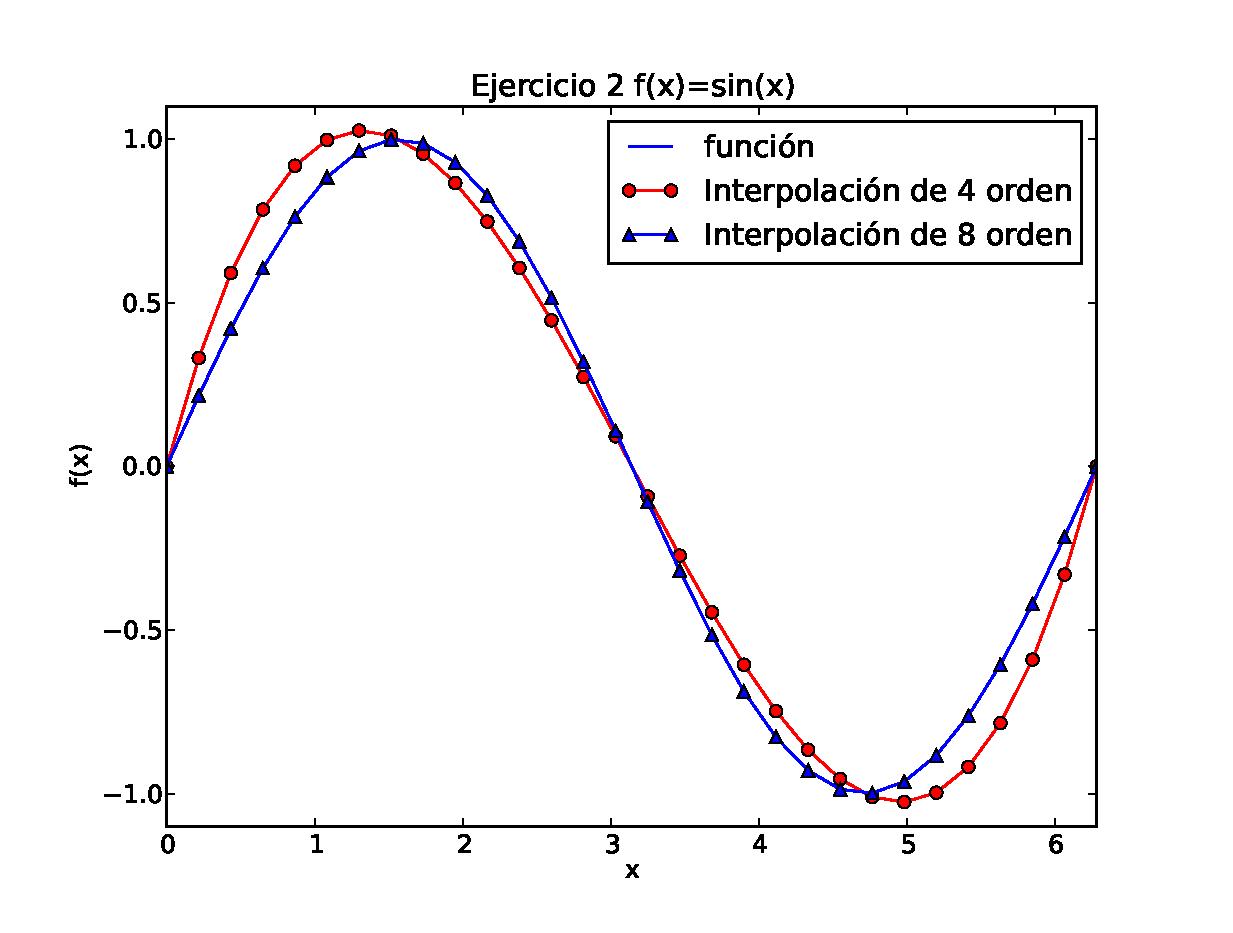
\includegraphics[scale=0.45]{Imagenes/ejercicioTema21_2.eps} 
\end{figure}
\end{frame}

\section{Consideraciones importantes}
\frame{\tableofcontents[currentsection, hideothersubsections]}
\subsection{Ventajas}

\begin{frame}
\frametitle{Consideraciones importantes}
La técnica de interpolación de Lagrange supone que el espaciamiento entre los puntos es la misma, por lo que cuando se presentan puntos que no cumplen ésta condición, la técnica ya no aplicaría.
\end{frame}

\subsection{Desventajas}

\begin{frame}
\frametitle{Desventajas interpolación de Lagrange}
A continuación se presentan algunas de las desventajas de la primera técnica de interpolación, al interpolación de Lagrange que hemos estudiado.
\end{frame}
\begin{frame}
\frametitle{Desventajas interpolación Lagrange}
\begin{itemize}[<+->]
\item[\ding{212}] La cantidad de cálculos necesarios para una interpolación es grande.
\item[\ding{212}] La interpolación para otro valor de $x$ necesita la misma cantidad de cálculos adicionales, ya que no se pueden utilizar partes de la aplicación previa.
\end{itemize}
\end{frame}
\begin{frame}
\frametitle{Desventajas interpolación Lagrange}
\begin{itemize}[<+->]
\item[\ding{212}] Cuando el número de datos tiene que incrementarse o decrementarse, no se pueden utilizar los resultados de los cálculos previos.
\item[\ding{212}] La evaluación del error no es fácil.
\end{itemize}
\pause
¿Cómo mejoramos el procedimiento de interpolación?
\end{frame}

\section{Interpolación de Newton}
\frame{\tableofcontents[currentsection, hideothersubsections]}
\subsection{Definición}

\begin{frame}
\frametitle{Interpolación de Newton}
Aunque el método de interpolación de Lagrange es conceptualmente sencillo, no es en sí, un algoritmo eficiente.
\\
\medskip
\pause
Un mejor método computacional se obtiene con el \textoazul{Método de Newton}.
\end{frame}
\begin{frame}
\frametitle{Interpolación de Newton}
El polinomio de interpolación de Newton se escribe de la forma:
\pause
\begin{align*}
P_{n} (x) &= a_{0} + (x - x_{0}) \: a_{1} + (x - x_{0})(x - x_{1}) \: a_{2} + \ldots + \\
&+ (x - x_{0})(x - x_{1}) \ldots (x - x_{n - 1}) \: a_{n} 
\end{align*}
\pause
Este polinomio nos permite contar con un procedimiento de evaluación más eficiente.
\end{frame}
\begin{frame}
\frametitle{Evaluación más eficiente}
Por ejemplo, con cuatro pares de datos ($n = 3$), tenemos que el polinomio de interpolación de Newton es:
\begin{align*}
P_{3}(x) &= a_{0} + (x - x_{0}) \: a_{1} (x - x_{0})(x - x_{1}) \: a_{2} + \\		
&+ (x - x_{0})(x - x_{1})(x - x_{2}) \: a_{3}
\end{align*}
\pause
Factorizando los términos, encontramos que:
\begin{align*}
P_{3} (x) &= a_{0} + \\
&+ (x - x_{0}) \left\{ a_{1}+(x - x_{1}) \left[ a_{2} + (x - x_{2}) \, a_{3} \right] \right\}
\end{align*}
\end{frame}
\begin{frame}
\frametitle{Evaluación del polinomio}
Que puede ser evaluado hacia atrás con las siguientes relaciones de recurrencia:
\pause
\begin{eqnarray*}
\begin{aligned}
P_{0} &= a_{3} \\ \pause
P_{1} &= a_{2} + (x - x_{2}) \: P_{0}(x) \\ \pause
P_{2} &= a_{1} + (x - x_{1}) \: P_{1}(x) \\ \pause
P_{3} &= a_{0} + (x - x_{0}) \: P_{2}(x) 
\end{aligned}
\end{eqnarray*}
\end{frame}
\begin{frame}
\frametitle{Evaluación del polinomio}
Para un $n$ arbitrario, tenemos:
\pause
\visible<2->{
\begin{align}
\begin{aligned}
P_{0} (x) =& \: a_{n} \\
P_{k} =& \: a_{n - k} + (x - x_{n - k}) \: P_{k - 1}(x), \hspace{0.5cm} k = 1,2,\ldots,n
\end{aligned}
\label{eq:ecuacion_03_04}
\end{align}
}
\end{frame}
\begin{frame}
\frametitle{Implementando un código en \python}
Una vez que ya se revisó la manera en la que podemos evaluar el polinomio de Newton, el siguiente paso es implementar un código en \python, para ello debemos de identificar los elementos con los que contamos al inicio de nuestro problema.
\end{frame}
\begin{frame}[fragile]
\frametitle{Estructurando el código en \python}
Definimos:
\setbeamercolor{item projected}{bg=aqua,fg=black}
\setbeamertemplate{enumerate items}{%
\usebeamercolor[bg]{item projected}%
\raisebox{1.5pt}{\colorbox{bg}{\color{fg}\footnotesize\insertenumlabel}}%
}
\begin{enumerate}[<+->]
\item Una variable $n$ que determina el grado del polinomio 
\item Un arreglo \texttt{xDatos} para las coordenadas $x$.
\item Un arreglo \texttt{yDatos} para las coordenadas $y$.
\item Un arreglo $a$ para almacenar los coeficientes del polinomio.
\end{enumerate}
\end{frame}
\begin{frame}[fragile]
\frametitle{Estructurando el código en \python}
Podemos usar el siguiente algoritmo para calcular $P_{n} (x)$:
\begin{lstlisting}[caption=Algoritmo para calcular $P_{n}$]
p = a[n]

for k in range(1, n + 1):
    p = a[n-k] + (x - xDatos[n-k]) * p
\end{lstlisting}
\end{frame}
\begin{frame}
\frametitle{Coeficientes del polinomio}
Los coeficientes de $P_{n}$ se calculan forzando que el polinomio pase a través del conjunto de puntos $y_{i} = P_{n} (x_{i}),\hspace{0.5cm} i = 0, 1, \ldots, n$. 
\end{frame}
\begin{frame}
\frametitle{Coeficientes del polinomio}
De tal manera que tenemos un sistema de ecuaciones simultáneas:
\pause
\begin{align*}
y_{0} &= a_{0} \\
y_{1} &= a_{0} + (x_{1} - x_{0}) \: a_{1} \\
y_{2} &= a_{0} + (x_{2} - x_{0}) \: a_{1} + (x_{2} - x_{0})(x_{2} - x_{1}) \: a_{2} \\
\vdots \\
y_{n} &= a_{0} + (x_{n} - x_{0}) \: a_{1} + \ldots + \\
&+ (x_{n} - x_{0})(x_{n} - x_{1}) \ldots (x_{n} - x_{n - 1}) \: a_{n}
\end{align*}
\end{frame}

\subsection{Diferencias divididas}

\begin{frame}[fragile]
\frametitle{Diferencias divididas}
Se introducen las diferencias divididas, de la siguiente forma:
\pause
\begin{eqnarray*}
\begin{aligned}
\nabla y_{i} &= \dfrac{y_{i} - y_{0}}{x_{i} - x_{0}}, \hspace{1cm} i = 1, 2, \ldots, n \\ \pause
\nabla^{2} y_{i} &= \dfrac{\nabla y_{i} - \nabla y_{1}}{x_{i} - x_{1}}, \hspace{1cm} i = 1,2,\ldots,n \\ \pause
\nabla^{3} y_{i} &= \dfrac{\nabla^{2} y_{i} - \nabla^{2} y_{2}}{x_{i} - x_{2}}, \hspace{1cm} i = 1,2,\ldots,n \\ \pause
\vdots \\ \pause
\nabla^{n} y_{i} &= \dfrac{\nabla^{n-1} y_{n} - \nabla^{n-1} y_{n-1}}{x_{n} - x_{n-1}}
\end{aligned}
\end{eqnarray*}
\end{frame}
\begin{frame}
\frametitle{Orden de las diferencias divididas}
Se puede hacer referencia al orden de las diferencias divididas:
\pause
\begin{eqnarray*}
\begin{aligned}
\nabla y_{i} & \hspace{0.5cm} \rightarrow \hspace{0.5cm} \text{Diferencias de orden 1} \\  \pause
\nabla^{2} y_{i} & \hspace{0.5cm} \rightarrow \hspace{0.5cm} \text{Diferencias de orden 2} \\ \pause
\vdots \\ \pause
\nabla^{n} y_{i} & \hspace{0.5cm} \rightarrow \hspace{0.5cm} \text{Diferencias de orden } n
\end{aligned}
\end{eqnarray*}
\pause
La letra delta invertida no refiere a un operador diferencial, sólo es una manera de expresar una diferencia, así como el exponente no implica una potenciación.
\end{frame}
\begin{frame}
\frametitle{Diferencias divididas}
La solución al sistema de ecuaciones es entonces:
\pause
\begin{eqnarray*}
\begin{aligned}
a_{0} &= y_{0} \\ \pause
a_{1} &= \nabla y_{1} \\ \pause
a_{2} &= \nabla^{2} y_{2} \\ \pause
\vdots \\ \pause
a_{n} &= \nabla^{n} y_{n}
\end{aligned}
\end{eqnarray*}
\end{frame}
\begin{frame}
\frametitle{Diferencias divididas}
Si los coeficientes se calculan a mano, es convieniente escribirlos con el siguiente formato:
(con $n=4$)
\pause
\begin{table}
\centering
\small
\begin{tabular}{| c | c | c | c | c | c |}
\hline $x_{0}$ & $y_{0}$ & & & & \\
\hline $x_{1}$ & $y_{1}$ & $\nabla y_{1}$ & & & \\
\hline $x_{2}$ & $y_{2}$ & $\nabla y_{2}$ & $\nabla^{2} y_{2}$ & &  \\
\hline $x_{3}$ & $y_{3}$ & $\nabla y_{3}$ & $\nabla^{2} y_{3}$ & $\nabla^{3} y_{3}$ &  \\
\hline $x_{4}$ & $y_{4}$ & $\nabla y_{4}$ & $\nabla^{2} y_{4}$ & $\nabla^{3} y_{4}$ & $\nabla^{4} y_{4}$ \\
\hline
\end{tabular}
\end{table}
\end{frame}
\begin{frame}
\frametitle{Diferencias divididas}
\textoazul{Los términos en la diagonal}
\begin{align*}
(y_{0}, \nabla y_{1}, \nabla^{2} y_{2}, \nabla^{3} y_{3}, \nabla^{4} y_{4})
\end{align*}
\pause
\textoazul{son los coeficientes del polinomio}.
\end{frame}
\begin{frame}
\frametitle{Diferencias divididas}
Si los puntos de datos se enumeran en un orden diferente, las entradas de la tabla van a cambiar, pero el polinomio resultante será el mismo.
\\
\bigskip
Recordemos que un polinomio de interpolación de grado $n$ con $n + 1$ datos diferentes, es único.
\end{frame}
\begin{frame}[fragile]
\frametitle{Estructurando el código}
Las operaciones en la computadora se pueden realizar con un arreglo unidimensional $a$, usando el siguiente algoritmo (tomando la notación $m = n + 1$ = número de puntos):
\end{frame}
\begin{frame}[fragile]
\frametitle{Estructurando el código}
\begin{lstlisting}[caption=Calculando los coeficientes del polinomio]
a = yDatos.copy()

for k in range(1, m):
    for i in range(k, m):
        a[i] = (a[i] - a[k-1])/(xDatos[i] - xDatos[k-1])
\end{lstlisting}
La función \texttt{.copy()} hace una copia del arreglo, dejando sin cambios en este caso al arreglo \texttt{yDatos}.
\end{frame}
\begin{frame}
\frametitle{Estructurando el código}
Inicialmente el arreglo $a$ contiene las coordenadas $y$ del conjunto de datos, es decir, la segunda columna de la tabla.
\end{frame}
\begin{frame}
\frametitle{Estructurando el código}
Cada vez que pasa por el bucle externo, se genera la siguiente columna, por lo que se sobreescriben los elementos de $a$, por tanto, al concluir el bucle, $a$ contiene los elementos de la diagonal, que son los coeficientes del polinomio.
\end{frame}

\subsection*{Usando un módulo con \python}

\begin{frame}
\frametitle{Usando un módulo con \python}
Para facilitar el mantenimiento y la lectura cuando los programas son demasiado largos, es posible \enquote{dividirlos} en \textocolor{blue}{módulos}, agrupando elementos relacionados.
\end{frame}

\subsection{Módulo \texttt{newtonPoli}}

\begin{frame}
\frametitle{Módulo \texttt{newtonPoli}}
El módulo \funcionazul{newtonPoli} incluye dos funciones que se requieren para la interpolación de Newton.
\setbeamercolor{item projected}{bg=beige,fg=bistre}
\setbeamertemplate{enumerate items}{%
\usebeamercolor[bg]{item projected}%
\raisebox{1.5pt}{\colorbox{bg}{\color{fg}\footnotesize\insertenumlabel}}%
}
\begin{enumerate}[<+->]
\item La función \funcionazul{coeffts}.
\item La función \funcionazul{evalPoli}
\end{enumerate}
\end{frame}
\begin{frame}
\frametitle{La función \funcionazul{coeffts}}
Dados el conjuntos de puntos en los arreglos \texttt{xDatos} y \texttt{yDatos}, la función \funcionazul{coeffts} devuelve el arreglo $a$ con los coeficientes.
\end{frame}
\begin{frame}
\frametitle{La función \funcionazul{evalPoli}}
Una vez que ya conocemos los coeficientes, el polinomio $P_{n}(x)$ puede evaluarse para cualquier valor de $x$ con la función \funcionazul{evalPoli}.
\end{frame}
\begin{frame}[fragile]
\frametitle{Código del módulo}
\begin{lstlisting}[caption=Funciones \texttt{coeffts} del módulo \texttt{newtonPoli}]    
def coeffts(xDatos, yDatos):
    m = len(xDatos) 
    a = yDatos.copy()
    for k in range(1, m):
        a[k:m] = (a[k:m] - a[k-1])/(xDatos[k:m] - xDatos[k-1])
    return a
\end{lstlisting}
\end{frame}
\begin{frame}[fragile]
\frametitle{Código del módulo}
\begin{lstlisting}[caption=Funciones \texttt{evalPoli} del módulo \texttt{newtonPoli}]
def evalPoli(a, xDatos, x):
    n = len(xDatos) - 1 
    p = a[n]

    for k in range(1, n+1):
        p = a[n-k] + (x - xDatos[n-k]) * p
    return p
\end{lstlisting}
\end{frame}
\begin{frame}
\frametitle{Resolviendo un ejemplo}
Ya contamos con los elementos necesarios para resolver un ejemplo, veamos a continuación el planteamiento del problema y su solución con \python.
\end{frame}
\begin{frame}
\frametitle{Ejercicio para resolver}
Los datos que se muestran en la siguiente tabla:
\pause
\begin{table}[H]
\small
\begin{tabular}{c | c | c | c | c | c | c}
$x$ & $0.15$ & $2.30$ & $3.15$ & $4.85$ & $6.25$ & $7.95$ \\ \hline
$y$ & $4.79867$ & $4.49013$ & $4.2243$ & $3.47313$ & $2.66674$ & $1.51909$
\end{tabular}
\end{table}
Se obtuvieron de la función:
\begin{align*}
f (x) = 4.8 \: \cos \left( \dfrac{\pi \: x}{20} \right)
\end{align*}
\end{frame}
\begin{frame}
\frametitle{Graficando los puntos iniciales}
\begin{figure}
    \centering
    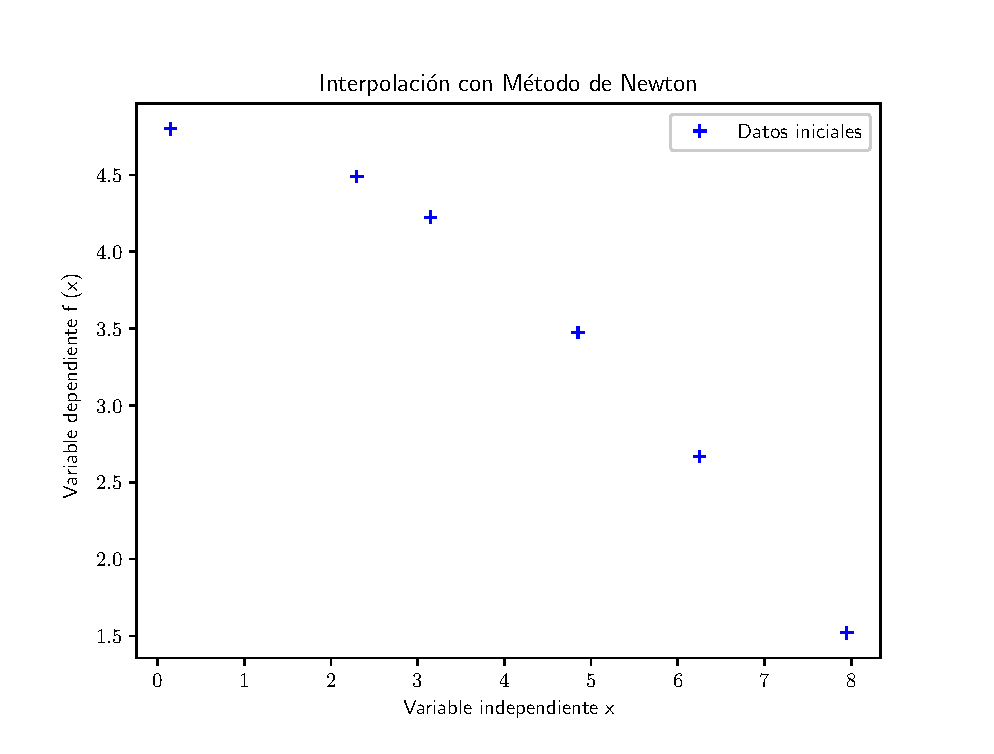
\includegraphics[scale=0.58]{Imagenes/Ejercicio_Newton_01.eps}
\end{figure}
\end{frame}    
\begin{frame}
\frametitle{Ejercicio para resolver}
Con ese conjunto de datos, interpola mediante el polinomio de Newton en los siguientes puntos:
\pause
\begin{align*}
x = 0, 0.5, 1.0, 1.5, \ldots, 7.5, 8.0
\end{align*}
\\
\bigskip
Compara los resultados con el valor \enquote{exacto} de los valores $y_{i} = f(x_{i})$, es decir, estima el error relativo.
\end{frame}
\begin{frame}[fragile]
\frametitle{Solución al ejercicio}
¿Qué necesitamos?
\\
\medskip
\pause
En un archivo nuevo en Spyder, llamamos a la librería \funcionazul{numpy} y también al módulo \funcionazul{newtonPoli} que contiene las funciones para resolver el polinomio de interpolación, también necesitaremos una función \funcionazul{errorRelativo} para comparar los valores exactos con los obtenidos.
\end{frame}
\begin{frame}[fragile]
\frametitle{Llamada a las librerías}
\begin{lstlisting}[caption=Llamando a las librerías y módulos]
import numpy as np
from newtonPoli import coeffts, evalPoli
\end{lstlisting}
\end{frame}
\begin{frame}[fragile]
\frametitle{Definiendo los arreglos}
Hay que crear los arreglos \texttt{xDatos} y \texttt{yDatos}, el arreglo $a$ se obtiene de la función \funcionazul{coeffts}.
\pause
\begin{lstlisting}[caption=Arreglos de la tabla]
xDatos = np.array([0.15,2.3,...,7.95])
yDatos = np.array([4.79867,4.49013,...,1.51909])
a = coeffts(xDatos, yDatos)
\end{lstlisting}
Recuerda que se deben de introducir todos los datos de la tabla.
\end{frame}
\begin{frame}[fragile]
\frametitle{Evaluación de los puntos}
La siguiente parte es proporcionar el rango de puntos en donde queremos evaluar mediante el método de Newton, a través de la función \funcionazul{evalPoli}:
\end{frame}
\begin{frame}[fragile]
\frametitle{Evaluación de los puntos}
\begin{lstlisting}[caption=Evaluando los puntos y el error relativo]
for x in np.arange(0.0, 8.1, 0.5):
    y = evalPoli(a, xDatos, x)
    print('{:1.1f} \t {:1.5f} \t {:1.5f} \t {:1.5E}'.format(x, y, yExacta, errorRelativo(yExacta, y)))
    # Falta almacenar los datos x, y 
    # para graficar los puntos interpolados
\end{lstlisting}
\end{frame}
\begin{frame}
\frametitle{Resultados obtenidos}
\begin{table}
\small
\centering
\renewcommand{\arraystretch}{0.9}
\begin{tabular}{l l l l}
x & yInterp & yExacta & ErrorRel\\ \hline
%\multicolumn{4}{l}{----------------------------------------} \\
$0.0$ & $4.80003$ & $4.80000$ & $5.22802E-04$ \\
$0.5$ & $4.78518$ & $4.78520$ & $5.16392E-04$ \\
$1.0$ & $4.74088$ & $4.74090$ & $5.70846E-04$ \\
$1.5$ & $4.66736$ & $4.66738$ & $3.19661E-04$ \\
\vdots \\
$7.0$ & $2.17915$ & $2.17915$ & $3.43797E-04$ \\
$7.5$ & $1.83687$ & $1.83688$ & $6.76648E-04$ \\
$8.0$ & $1.48329$ & $1.48328$ & $2.67576E-04$
\end{tabular}
\end{table}
\end{frame}
\begin{frame}
\frametitle{Graficando los puntos iniciales e interpolados}
\begin{figure}
    \centering
    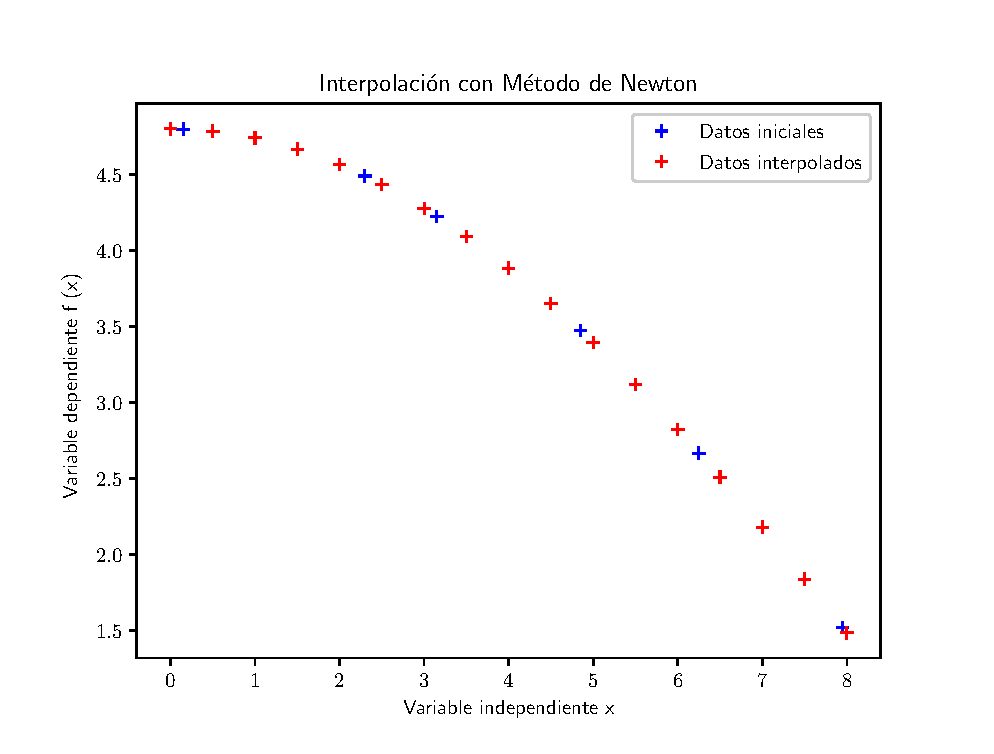
\includegraphics[scale=0.58]{Imagenes/Ejercicio_Newton_02.eps}
\end{figure}
\end{frame}
\begin{frame}
\frametitle{Agregando elementos}
Nuevamente en el enunciado del problema no se pide una gráfica, pero podemos aportar una y con ella discutir la congruencia de los resultados obtenidos.
\\
\bigskip
\pause
Es una buena idea contar con una función que grafique los resultados, ya contamos con lo necesario para ello.
\end{frame}
\begin{frame}
\frametitle{Graficando todo al mismo tiempo}
Tenemos lo siguiente:
\setbeamercolor{item projected}{bg=blue,fg=blond}
\setbeamertemplate{enumerate items}{%
\usebeamercolor[bg]{item projected}%
\raisebox{1.5pt}{\colorbox{bg}{\color{fg}\footnotesize\insertenumlabel}}%
}
\begin{enumerate}[<+->]
\item Los datos iniciales.
\item Los datos interpolados, que ya se debieron de haber almacenado en un objeto de \python.
\item Vamos a evaluar la \textit{función exacta} en el intervalo $[0, 8]$ para mostrar la gráfica, necesitaremos una función que evalúe los datos del intervalo.
\end{enumerate}
\end{frame}
\begin{frame}[allowframebreaks, fragile]
\frametitle{Función y rutina de graficación}
Dejamos la función en la parte superior del código, para luego usar la rutina de graficación tradicional:
\begin{lstlisting}[caption=Graficando la función exacta]
def yExacta(x):
    valor = 4.8 * np.cos(np.pi * x/20.0)
    return valor

x2 = np.linspace(0, 8)

plt.plot(x2, yExacta(x2), 'k', lw=0.7, ls='dashed', label=u'Funcion exacta')
\end{lstlisting}
\end{frame}
\begin{frame}
\frametitle{Completando la gráfica}
Revisa que la gráfica que se presenta tiene más elementos a modo de \enquote{decoradores}: \pause etiquetas en los ejes, título, leyenda de identificación, estilo de línea, color, etc.
\\
\bigskip
\pause
Le puedes dedicar otro momento para completar esa información que siempre es de utilidad, revisa la documentación de \funcionazul{matplotlib} y encontrarás bastantes cosas prácticas.
\end{frame}
\begin{frame}
\frametitle{Graficando los puntos y la función $f (x)$}
\begin{figure}
    \centering
    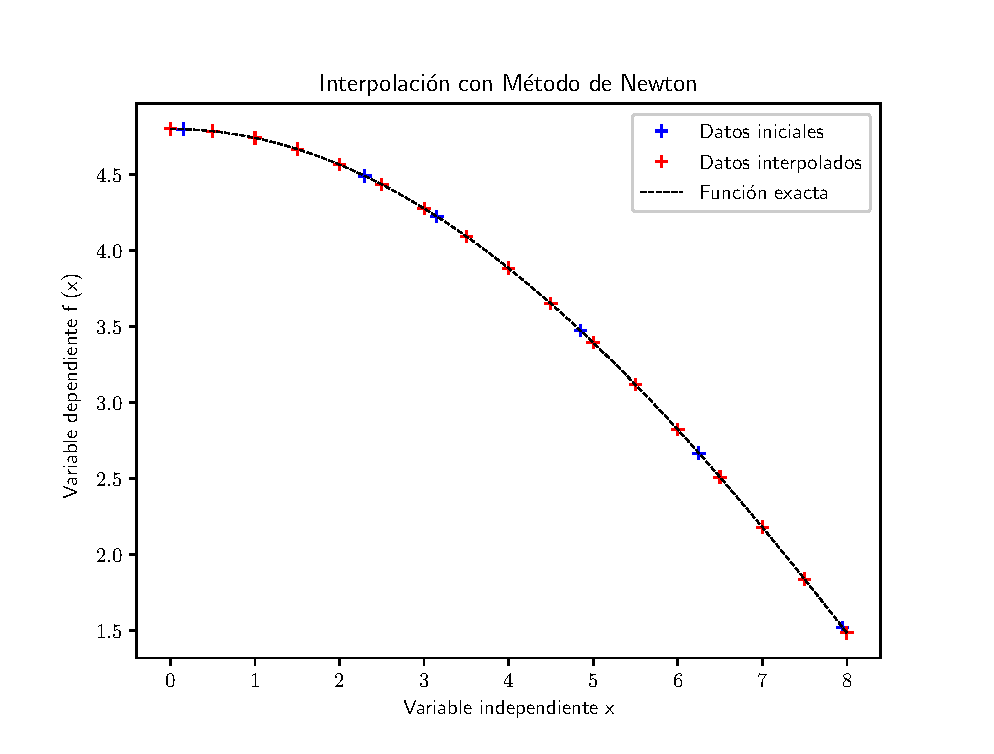
\includegraphics[scale=0.58]{Imagenes/Ejercicio_Newton_03.eps}
\end{figure}
\end{frame}
\end{document}